% =========================================================================
%  Fast, efficient, VRAM-friendly LLM serving
%  MiRA Training Course 2026 - 9/4, 10:20-11:00, R546
%
%  Build:   tectonic llm_serving_talk.tex
%  (also compiles with:  lualatex llm_serving_talk.tex  x2 )
%
%  Speaker notes: uncomment ONE of the \setbeameroption lines below.
% =========================================================================
\documentclass[aspectratio=169,10pt]{beamer}

\usetheme{metropolis}
\metroset{numbering=fraction, progressbar=foot, block=fill}

% --- Fonts: XeTeX/LuaTeX get a CJK family for the speaker's name ----------
\usepackage{iftex}
\ifXeTeX
  \usepackage{fontspec}
  \IfFontExistsTF{Noto Sans CJK TC}{%
    \newfontfamily\cjkfamily{Noto Sans CJK TC}%
    \newcommand{\CJK}[2]{{\cjkfamily #1}}%
  }{%
    \IfFontExistsTF{Noto Sans CJK SC}{%
      \newfontfamily\cjkfamily{Noto Sans CJK SC}%
      \newcommand{\CJK}[2]{{\cjkfamily #1}}%
    }{\newcommand{\CJK}[2]{#2}}%
  }
\else\ifLuaTeX
  \usepackage{fontspec}
  \IfFontExistsTF{Noto Sans CJK TC}{%
    \newfontfamily\cjkfamily{Noto Sans CJK TC}%
    \newcommand{\CJK}[2]{{\cjkfamily #1}}%
  }{\newcommand{\CJK}[2]{#2}}
\else
  % pdflatex has no system-font access: fall back to the Latin transcription
  \usepackage[T1]{fontenc}
  \usepackage[utf8]{inputenc}
  \newcommand{\CJK}[2]{#2}
\fi\fi
% Usage: \CJK{<CJK text>}{<Latin fallback>}

\usepackage{amsmath, amssymb, mathtools}
\usepackage{booktabs}
\usepackage{graphicx}
\usepackage{tikz}
\usetikzlibrary{arrows.meta, positioning, fit, backgrounds, calc, decorations.pathreplacing}
\usepackage{url}

\definecolor{accent}{HTML}{1F6FEB}
\definecolor{warn}{HTML}{C2410C}
\definecolor{good}{HTML}{15803D}
\newcommand{\emphc}[1]{\textcolor{accent}{\textbf{#1}}}
\newcommand{\warnc}[1]{\textcolor{warn}{\textbf{#1}}}
\newcommand{\goodc}[1]{\textcolor{good}{\textbf{#1}}}

% --- Badges ---------------------------------------------------------------
\newcommand{\demo}[1]{%
  \tikz[baseline=(x.base)]\node[fill=good, text=white, rounded corners=2pt,
        inner xsep=4pt, inner ysep=1.5pt, font=\bfseries\scriptsize] (x)
        {LIVE DEMO: notebook #1};}
\newcommand{\cutbadge}[1]{%
  \tikz[baseline=(x.base)]\node[fill=warn, text=white, rounded corners=2pt,
        inner xsep=4pt, inner ysep=1.5pt, font=\bfseries\scriptsize] (x)
        {CUT #1};}

% --- Speaker notes: uncomment to render -----------------------------------
% \setbeameroption{show notes}
% \setbeameroption{show notes on second screen=right}

\title{Fast, efficient, VRAM-friendly LLM serving}
\subtitle{Memory decides serving cost, and you can compute it in advance}
\author{\CJK{仲翊}{Chung-Yi}}
\institute{MiRA Training Course 2026}
\date{9/4, 10:20--11:00 \quad R546}

\begin{document}

% =========================================================================
\maketitle
\note{\textbf{0:00.} Name, and the promise: 40 minutes, and you leave able to
size a deployment on paper. Inference only, no architecture. Say the end time: 11:00.}

% -------------------------------------------------------------------------
\begin{frame}{``Put this model on our machine.'' Does it fit?}
  \begin{block}{Your advisor, some time in the next twelve months}
    ``Put this model on our machine so the lab can use it.''
  \end{block}
  \vspace{0.5em}
  You have \emphc{one GPU}. The model is \emphc{70B parameters}.
  \begin{itemize}
    \item Does it fit?
    \item If it fits, how many people can use it at once?
    \item If it is too slow, what do you change \emph{first}?
  \end{itemize}
  \vspace{0.6em}
  \uncover<2->{\warnc{Most people answer this by trial and error.}}
\end{frame}
\note{\textbf{0:30.} Show of hands: who has downloaded a model and hoped it would
load? Everyone.}

% -------------------------------------------------------------------------
\begin{frame}{It is arithmetic, and by 11:00 you will be able to do it}
  \begin{alertblock}{The one thing}
    \textbf{Memory decides serving cost.}
    Compute the VRAM budget and the memory-bandwidth ceiling, and each
    deployment decision (quantize, batch, shrink, or buy another GPU)
    follows from arithmetic.
  \end{alertblock}
  \vspace{0.4em}
  Three questions, three pieces of arithmetic:
  \begin{enumerate}
    \item \textbf{Does it fit?} $\rightarrow$ the VRAM budget
    \item \textbf{How fast can it possibly go?} $\rightarrow$ the bandwidth ceiling
    \item \textbf{Which knob do I turn?} $\rightarrow$ a ranked toolbox
  \end{enumerate}
\end{frame}
\note{\textbf{1:30.} Point at the map once. We need one fact about attention, and it
arrives in Movement 1.}

% -------------------------------------------------------------------------
\begin{frame}[fragile]{Every number on these slides is a cell you can run}
  \begin{center}
    {\small\url{github.com/Chung-I/MiRA_training_course_2026}}\\[0.3em]
    {\footnotesize click the Colab badge next to
     \texttt{notebooks/llm\_serving\_demo.ipynb}}\\[0.5em]
    {\tiny\url{https://colab.research.google.com/github/Chung-I/MiRA_training_course_2026/blob/main/notebooks/llm_serving_demo.ipynb}}
  \end{center}
  \vspace{0.4em}
  \begin{columns}[T]
    \begin{column}{0.48\textwidth}
      \textbf{Parts 1--5: no GPU, no installs}\\
      \small Pure standard library. VRAM, KV cache, bandwidth and cost
      calculators. This is the arithmetic half.
    \end{column}
    \begin{column}{0.48\textwidth}
      \textbf{Parts 6--8: needs a GPU}\\
      \small Colab free T4 is enough
      (\texttt{Runtime $\rightarrow$ Change runtime type}).
      Measures the predictions against a real card.
    \end{column}
  \end{columns}
  \vspace{0.8em}
  \begin{center}
    \demo{Part 7} \quad and \quad \demo{Part 8} \quad are run live, later.
  \end{center}
\end{frame}
\note{\textbf{2:30.} Open the tab now and leave it open. Do not install
anything live. Say: you can follow along, but you will get more out of
watching first and running it on the train home.}

% =========================================================================
\section{The VRAM budget}
% =========================================================================

\begin{frame}{Four things live in your VRAM. You forget one of them.}
  \vspace{0.5em}
  \begin{center}\Large
    weights \;$+$\; \emphc{KV cache} \;$+$\; activations \;$+$\;
    framework overhead
  \end{center}
  \vspace{1.0em}
  \begin{itemize}
    \item \textbf{Weights}: a fixed cost, paid once, easy to compute.
    \item \emphc{KV cache}: paid \emph{per user, per token}. Few people compute it.
    \item \textbf{Activations}: small at inference; batch-dependent.
    \item \textbf{Overhead / fragmentation}: allocator, CUDA context, workspace.
          Budget $\approx$ 2\,GB and stop worrying.
  \end{itemize}
  \vspace{0.6em}
  \uncover<2->{The first two set the budget. Most of this talk is about the second.}
\end{frame}
\note{\textbf{3:30.} Fragmentation gets a whole slide of its own later.
PagedAttention exists to remove it.}

% -------------------------------------------------------------------------
\begin{frame}{Weights $=$ parameters $\times$ bytes. 70B in fp16 is 140\,GB.}
  \begin{equation*}
    \text{weight bytes} \;=\; \text{parameters} \times \text{bytes per parameter}
  \end{equation*}
  \begin{center}\small
    fp32 $=4$ \quad fp16 / bf16 $=2$ \quad fp8 / int8 $=1$ \quad int4 $=0.5$
  \end{center}
  \vspace{0.4em}
  \begin{center}
    \begin{tabular}{lrrr}
      \toprule
      model & fp16 & int8 & int4 \\
      \midrule
      8B  &  16\,GB &  8\,GB & 4\,GB \\
      \textbf{70B} & \warnc{140\,GB} & 70\,GB & \emphc{35\,GB} \\
      405B & 810\,GB & 405\,GB & 203\,GB \\
      \bottomrule
    \end{tabular}
  \end{center}
  \vspace{0.5em}
  \warnc{140\,GB} fits on no card you own.
  \emphc{35\,GB} fits on one 40\,GB card, barely.
  \textbf{That row decides the deployment architecture.}
\end{frame}
\note{\textbf{4:30.} Read the 70B row out loud. It is the cheapest useful
calculation in machine learning, and most people skip it before hitting
download.}

% -------------------------------------------------------------------------
\begin{frame}{The KV cache formula, which most people skip}
  \begin{equation*}
    \underbrace{\text{KV bytes per token}}_{\text{per user, per token}}
    \;=\;
    \underbrace{2}_{\mathclap{\text{K and V}}}
    \;\times\; \text{layers}
    \;\times\; \text{kv\_heads}
    \;\times\; \text{head\_dim}
    \;\times\; \text{bytes per value}
  \end{equation*}
  \vspace{1.2em}
  \begin{itemize}
    \item Every token you have already generated stays in memory.
    \item It grows \emph{linearly} with conversation length.
    \item It is charged \emph{once per concurrent user}.
  \end{itemize}
  \vspace{0.6em}
  \emphc{Four numbers, all of them in the model's \texttt{config.json}.}
\end{frame}
\note{\textbf{5:30.} The one fact about attention I assume: decoding needs the keys
and values of every previous token, so you keep them.}

% -------------------------------------------------------------------------
\begin{frame}{Llama-3-8B: 128\,KiB per token, 1\,GiB per conversation}
  \textbf{Llama-3-8B:} 32 layers, 8 KV heads, head\_dim 128, fp16 cache.
  \vspace{0.6em}
  \begin{align*}
    \text{KV per token}
      &= 2 \times 32 \times 8 \times 128 \times 2\ \text{bytes} \\[0.2em]
    \uncover<2->{&= 131{,}072\ \text{bytes} \;=\; \emphc{128\ \text{KiB per token}}} \\[0.6em]
    \uncover<3->{\text{An 8k conversation} &= 8192 \times 128\ \text{KiB}
      \;=\; \warnc{1\ \text{GiB} \ \text{for one user}}}
  \end{align*}
  \vspace{0.4em}
  \uncover<3->{You pay 16\,GB for the weights once. You pay this 1\,GiB again for
  each person who opens a chat window.}
\end{frame}
\note{\textbf{6:30.} Do the multiplication out loud, slowly. The whole
talk hangs on this slide. Pause after ``for one user''.}

% -------------------------------------------------------------------------
\begin{frame}{GQA is why you can serve modern models}
  \begin{center}
    \begin{tabular}{lrrr}
      \toprule
      model & KV heads & KV per token & 8k conversation \\
      \midrule
      Llama-2-7B \small(MHA) & 32 & \warnc{512\,KiB} & 4\,GiB \\
      Llama-3-8B \small(GQA) &  8 & \emphc{128\,KiB} & 1\,GiB \\
      \bottomrule
    \end{tabular}
  \end{center}
  \vspace{1.0em}
  \begin{center}\large
    The \emph{smaller} model costs \warnc{four times more cache per token.}
  \end{center}
  \vspace{0.8em}
  Only one thing changed: \emphc{Grouped-Query Attention} shares one set of
  K/V across several query heads, so \texttt{kv\_heads} drops from 32 to 8.
  Same formula, one quarter of the memory.
\end{frame}
\note{\textbf{7:30.} Parameter count is a bad proxy for servability. If
somebody asks ``is a 7B easier to serve than an 8B'', this is the answer:
check \texttt{num\_key\_value\_heads}, not the name.}

% -------------------------------------------------------------------------
\begin{frame}{Weights are a fixed cost. The KV cache is a per-user cost.}
  \vspace{1.2em}
  \begin{center}
    \begin{minipage}{0.86\textwidth}
      \begin{alertblock}{The consequence}
        Whatever VRAM is left \emph{after} the weights is what you divide
        among concurrent users.

        \vspace{0.4em}
        The \textbf{KV cache} sets your \textbf{throughput}.
      \end{alertblock}
    \end{minipage}
  \end{center}
  \vspace{1.0em}
  \begin{center}\large
    $\text{users} \;\approx\;
      \dfrac{\text{VRAM} - \text{weights} - \text{overhead}}
            {\text{KV per token} \times \text{context length}}$
  \end{center}
\end{frame}
\note{\textbf{8:30.} Say it twice. They should still have this sentence in a year.
Each tool in the toolbox shrinks the weights term or the denominator.}

% -------------------------------------------------------------------------
\begin{frame}{One 24\,GB card, one model: 7 users, or 36}
  \textbf{Llama-3-8B, 8k context per user, 24\,GB card, 2\,GB overhead.}
  \vspace{0.5em}
  \begin{center}
    \begin{tabular}{llrrr}
      \toprule
      weights & KV cache & weights & free & \textbf{concurrent users} \\
      \midrule
      fp16 & fp16 & 14.9\,GB & 7.1\,GB & \warnc{7} \\
      int4 & fp16 &  3.7\,GB & 18.3\,GB & 18 \\
      int4 & fp8  &  3.7\,GB & 18.3\,GB & \emphc{36} \\
      \bottomrule
    \end{tabular}
  \end{center}
  \vspace{0.8em}
  \begin{center}\large
    \textbf{Same GPU, same model, two flags: \emphc{five times the users.}}
  \end{center}
\end{frame}
\note{\textbf{9:30.} Notebook Part 3 prints this table for any card you name.
Quantizing the \emph{cache} pays as much as quantizing the weights once the
weights are small, and few people turn it on.
End of Movement 1. You should be at 10 minutes.}

% =========================================================================
\section{Why decoding is slow}
% =========================================================================

\begin{frame}{Prefill is compute-bound. Decode is bandwidth-bound.}
  \begin{columns}[T]
    \begin{column}{0.48\textwidth}
      \textbf{Prefill} (your prompt)\\[0.3em]
      \small All prompt tokens go through the network \emph{in parallel}.
      Big matrix multiplies, the GPU's arithmetic units are busy.
      \emph{Compute-bound.}
    \end{column}
    \begin{column}{0.48\textwidth}
      \textbf{Decode} (the answer)\\[0.3em]
      \small One token at a time, in sequence. Each token requires
      reading \emph{every weight} out of HBM. The GPU spends its time moving
      bytes. \emph{Bandwidth-bound.}
    \end{column}
  \end{columns}
  \vspace{1.0em}
  \begin{center}
    \begin{minipage}{0.9\textwidth}
      \begin{block}{The corollary you can charge money for}
        A 10k-token \emph{prompt} is cheap and 10k \emph{output} tokens are
        expensive. Prompt tokens run in parallel; output tokens wait in a queue.
      \end{block}
    \end{minipage}
  \end{center}
\end{frame}
\note{\textbf{10:00.} This fact explains the rest of the talk. The sentence to keep
from Movement 2: ``decoding reads all the weights, once per token''.}

% -------------------------------------------------------------------------
\begin{frame}{Your tokens/sec ceiling is bandwidth $\div$ bytes of weights}
  \begin{equation*}
    \text{tokens/sec} \;\leq\;
    \frac{\text{memory bandwidth}}{\text{bytes of weights read per token}}
  \end{equation*}
  \vspace{0.6em}
  \begin{itemize}
    \item An \textbf{upper bound}. Better code cannot beat it.
    \item 8B in fp16 reads \textbf{16\,GB} per token;
          in int4 it reads \textbf{4\,GB}.
          Same card, same math, \emphc{four times the ceiling}.
    \item \uncover<2->{Quantization speeds up decoding because it
          \emph{moves fewer bytes}. The arithmetic costs about the same.}
    \item \uncover<3->{Small models are \emph{disproportionately} fast:
          their bottleneck is their own size.}
  \end{itemize}
\end{frame}
\note{\textbf{11:30.} Kill the ``quantization is faster because fewer FLOPs''
folklore here. int4 arithmetic costs about the same; int4 \emph{traffic}
is 4x cheaper.}

% -------------------------------------------------------------------------
\begin{frame}{\texttt{generate()} reaches 9.4\% of the hardware}
  \hfill\demo{Part 6--7}
  \vspace{0.2em}

  \textbf{RTX 5090, Qwen2.5-0.5B, fp16.} First, does the arithmetic hold?
  \begin{center}\small
    \begin{tabular}{lrr}
      \toprule
      & predicted & measured \\
      \midrule
      weight memory & 0.920\,GB & 0.928\,GB \quad (ratio \emphc{1.008}) \\
      \bottomrule
    \end{tabular}
  \end{center}
  \vspace{0.6em}
  Then, how close to the roof does a plain for-loop get?
  \begin{center}\small
    \begin{tabular}{lr}
      \toprule
      bandwidth ceiling & 1811.6 tok/s \\
      HuggingFace \texttt{generate()} decode & \warnc{169.9 tok/s} \\
      \midrule
      \textbf{efficiency} & \warnc{9.4\% of the hardware} \\
      \bottomrule
    \end{tabular}
  \end{center}
  \vspace{0.4em}
  \emphc{That 90\% gap is the argument for a serving engine.}
\end{frame}
\note{\textbf{12:30.} Run this live. The 1.008 ratio earns their trust in the
arithmetic; the 9.4\% earns you Movement 3. \texttt{generate()} is a
correctness reference.}

% -------------------------------------------------------------------------
\begin{frame}{Batching is nearly free: 15$\times$ the throughput, 4\% slower per user}
  \hfill\demo{Part 8}
  \vspace{0.2em}

  The weights are read \emph{once for the whole batch}. So a bigger batch is
  almost pure profit.
  \begin{center}
    \begin{tabular}{rrrr}
      \toprule
      batch & total tok/s & per-user tok/s & wall time \\
      \midrule
       1 &  169.3 & 169.3 & 0.39\,s \\
      16 & \emphc{2594.6} & 162.2 & 0.39\,s \\
      \bottomrule
    \end{tabular}
  \end{center}
  \vspace{0.5em}
  \begin{center}\small RTX 5090, Qwen2.5-0.5B, 64 new tokens.\end{center}
  \vspace{0.4em}
  \begin{itemize}
    \item \textbf{Same wall-clock time.} Sixteen users served instead of one.
    \item \emphc{The KV cache} limits the batch, which takes us back to Movement 1.
  \end{itemize}
\end{frame}
\note{\textbf{13:30.} Run this live too, the most persuasive number in the talk.
Let the 0.39\,s column land: the sixteenth user cost you nothing. Cache
capacity is throughput.}

% -------------------------------------------------------------------------
\begin{frame}{Report TTFT, ITL and throughput together}
  \begin{center}
    \begin{tabular}{lll}
      \toprule
      \textbf{TTFT} & time to first token & prefill; what the user \emph{feels} \\
      \textbf{ITL / TPOT} & inter-token latency & decode; how fast text appears \\
      \textbf{Throughput} & total tok/s, all users & what you \emph{pay} for \\
      \bottomrule
    \end{tabular}
  \end{center}
  \vspace{1.0em}
  \begin{itemize}
    \item Latency and throughput \emph{trade against each other}.
          Batching improves one and worsens the other.
    \item \warnc{A benchmark without a stated concurrency level tells you nothing.}
    \item ``Our server does 2000 tok/s'': at what batch size, and with
          what TTFT?
  \end{itemize}
\end{frame}
\note{\textbf{15:00.} This slide saves them from a bad paper table. Three
numbers, together, with the concurrency.
End of Movement 2. You should be at 18 minutes.}

% =========================================================================
\section{The toolbox, in order of payoff}
% =========================================================================

\begin{frame}{The toolbox, ranked. The ranking is the content.}
  \begin{enumerate}\small
    \item \emphc{Use a real serving engine.} vLLM / SGLang / TensorRT-LLM.
          One-line change, largest single payoff.
    \item \emphc{Quantize the weights.} int4/int8/FP8. $\approx\frac14$ the VRAM,
          several times the decode speed.
    \item \emphc{Quantize the KV cache too.} fp8 or int8. Directly doubles
          your user count. Underused.
    \item \emphc{Cache the prefix.} Shared system prompt or retrieved
          documents: prefill once, reuse.
    \item Speculative decoding. 1.5--3$\times$, identical output distribution.
          \hfill\cutbadge{2: appendix}
    \item A smaller model, or one base $+$ many LoRA adapters.
          \hfill\cutbadge{2: appendix}
    \item More GPUs. \emph{Last.}
          \hfill\cutbadge{2: appendix}
  \end{enumerate}
  \vspace{0.3em}
  \begin{center}\small
    The order is what you take home.
  \end{center}
\end{frame}
\note{\textbf{18:00.} If you are behind schedule, this frame alone carries
items 5--7 and you skip their appendix slides entirely. Say the order out
loud; the order is the deliverable.}

% -------------------------------------------------------------------------
\begin{frame}{\#1 A real engine, because two features do all the work}
  \begin{columns}[T]
    \begin{column}{0.48\textwidth}
      \textbf{Continuous batching}\\[0.3em]
      \small A finished request \emph{leaves the batch immediately} instead
      of waiting for the slowest one in its group. New requests join on the
      next step. No head-of-line blocking.
    \end{column}
    \begin{column}{0.48\textwidth}
      \textbf{PagedAttention}\\[0.3em]
      \small The KV cache in fixed-size \emph{pages}, like OS virtual memory.
      Blocks need not be contiguous, and you stop reserving for the worst
      case.
    \end{column}
  \end{columns}
  \vspace{1.2em}
  \begin{center}
    \begin{minipage}{0.88\textwidth}
      \begin{alertblock}{}
        \centering
        Replacing \texttt{model.generate()} in a for-loop with
        \texttt{vllm serve} is \emph{a one-line change}, and it is the
        largest single win available to you.
      \end{alertblock}
    \end{minipage}
  \end{center}
\end{frame}
\note{\textbf{19:00.} They will be tempted to write their own batching loop.
Tell them plainly: you will get it wrong, and the people who got it right
gave it away.}

% -------------------------------------------------------------------------
\begin{frame}{PagedAttention: the KV cache as virtual memory}
\vspace{-0.2em}
\begin{center}
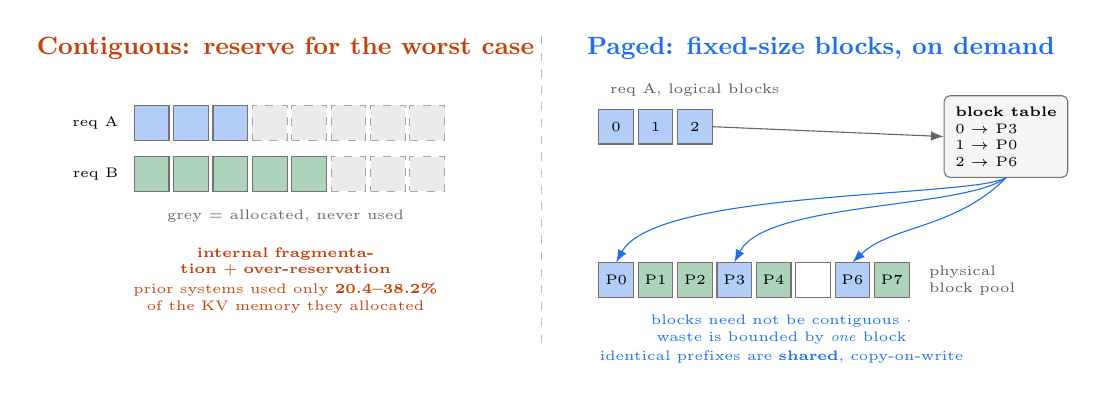
\begin{tikzpicture}[
  font=\scriptsize,
  blk/.style={draw=black!55, minimum width=0.44cm, minimum height=0.44cm,
              inner sep=0pt, font=\tiny},
  useA/.style={blk, fill=accent!35},
  useB/.style={blk, fill=good!35},
  waste/.style={blk, fill=black!8, dashed, draw=black!35},
  ttl/.style={font=\small\bfseries},
  ar/.style={-{Latex[length=1.6mm]}}
]

% ================= LEFT: contiguous allocation =================
\node[ttl, warn] at (2.3, 4.85) {Contiguous: reserve for the worst case};

\node[anchor=east, font=\tiny] at (0.30, 3.90) {req A};
\foreach \i in {0,1,2}   {\node[useA]  at (0.60+\i*0.50, 3.90) {};}
\foreach \i in {3,...,7} {\node[waste] at (0.60+\i*0.50, 3.90) {};}

\node[anchor=east, font=\tiny] at (0.30, 3.25) {req B};
\foreach \i in {0,...,4} {\node[useB]  at (0.60+\i*0.50, 3.25) {};}
\foreach \i in {5,6,7}   {\node[waste] at (0.60+\i*0.50, 3.25) {};}

\node[font=\tiny, black!60] at (2.30, 2.72)
  {grey $=$ allocated, never used};

\node[text width=4.7cm, align=center, font=\tiny, warn] at (2.30, 1.90)
  {\textbf{internal fragmentation $+$ over-reservation}\\[0.15em]
   prior systems used only \textbf{20.4--38.2\%}\\
   of the KV memory they allocated};

% ================= divider =================
\draw[black!25, dashed] (5.55, 1.10) -- (5.55, 5.10);

% ================= RIGHT: paged allocation =================
\node[ttl, accent] at (9.10, 4.85) {Paged: fixed-size blocks, on demand};

% --- logical blocks of request A ---
\node[anchor=west, font=\tiny, black!65] at (6.30, 4.32) {req A, logical blocks};
\node[useA] (LA0) at (6.50, 3.85) {0};
\node[useA] (LA1) at (7.00, 3.85) {1};
\node[useA] (LA2) at (7.50, 3.85) {2};

% --- block table ---
\node[draw=black!55, fill=black!4, rounded corners=2pt, align=left,
      font=\tiny, inner sep=4pt, anchor=north] (BT) at (11.45, 4.25)
  {\textbf{block table}\\ $0 \rightarrow$ P3\\ $1 \rightarrow$ P0\\ $2 \rightarrow$ P6};

\draw[ar, black!60] (LA2.east) -- (BT.west);

% --- physical block pool ---
\node[anchor=west, font=\tiny, black!65, align=left] at (10.35, 1.90)
  {physical\\ block pool};
\node[useA] (P0) at (6.50, 1.90) {P0};
\node[useB] (P1) at (7.00, 1.90) {P1};
\node[useB] (P2) at (7.50, 1.90) {P2};
\node[useA] (P3) at (8.00, 1.90) {P3};
\node[useB] (P4) at (8.50, 1.90) {P4};
\node[blk]  (P5) at (9.00, 1.90) {};
\node[useA] (P6) at (9.50, 1.90) {P6};
\node[useB] (P7) at (10.00, 1.90) {P7};

\draw[ar, accent] (BT.south) .. controls (11.0, 2.95) and (7.0, 3.05) .. (P0.north);
\draw[ar, accent] (BT.south) .. controls (10.9, 2.80) and (8.4, 2.90) .. (P3.north);
\draw[ar, accent] (BT.south) .. controls (10.8, 2.55) and (10.0, 2.60) .. (P6.north);

\node[text width=5.4cm, align=center, font=\tiny, accent] at (8.60, 1.15)
  {blocks need not be contiguous $\cdot$ waste is bounded by \emph{one} block\\[0.15em]
   identical prefixes are \textbf{shared}, copy-on-write};

\end{tikzpicture}
\end{center}
\vspace{-0.2em}
{\scriptsize Kwon et al., \emph{Efficient Memory Management for LLM Serving with
PagedAttention}, arXiv:2309.06180.}
\end{frame}
\note{\textbf{20:00.} The most important picture in the talk. Say the OS
analogy: these are page tables. Then the payoff: waste drops
from ``the whole unused tail'' to ``at most one block'', and two requests
with the same system prompt point at the same physical blocks.}

% -------------------------------------------------------------------------
\begin{frame}{\#2--3 Quantize the weights, then quantize the cache}
  \begin{columns}[T]
    \begin{column}{0.49\textwidth}
      \textbf{\#2 Weights}\\[0.3em]
      \small
      AWQ, GPTQ (post-training, weight-only); FP8 natively on Hopper and
      newer.\\[0.4em]
      $\approx \frac14$ the VRAM at 4-bit, and several times the decode speed
      because it moves fewer bytes.
    \end{column}
    \begin{column}{0.49\textwidth}
      \textbf{\#3 The KV cache}\\[0.3em]
      \small
      fp8 or int8 cache. Directly \emph{doubles} the number of users you can
      hold.\\[0.4em]
      It follows from Movement 1, and few people turn it on.
      In our table it was 18 users $\rightarrow$ \emphc{36}.
    \end{column}
  \end{columns}
  \vspace{1.2em}
  \begin{center}
    \begin{minipage}{0.88\textwidth}
      \begin{alertblock}{The rule}
        \centering
        Quality loss is small on most tasks and large on some.\\
        \textbf{Quantize, then re-run your own eval. A published perplexity
        tells you little.}
      \end{alertblock}
    \end{minipage}
  \end{center}
\end{frame}
\note{\textbf{21:30.} Do not survey quantization algorithms. Name AWQ, GPTQ,
FP8, give the rule, move on. If asked which: whatever your engine supports
for your card.}

% -------------------------------------------------------------------------
\begin{frame}{\#4 Prefix caching is free, and it is the biggest RAG win}
  \begin{itemize}
    \item Every request begins with the same 2000-token system prompt.
    \item Every RAG request begins with the same retrieved documents.
    \item \emphc{Prefill it once. Reuse the KV blocks for every later request.}
  \end{itemize}
  \vspace{1.0em}
  \begin{center}
    \begin{minipage}{0.88\textwidth}
      \begin{block}{Why it is nearly free}
        Those KV blocks already exist in memory, and PagedAttention already
        lets two requests point at the same physical block. Prefix caching is
        what paging \emph{buys} you.
      \end{block}
    \end{minipage}
  \end{center}
  \vspace{0.8em}
  It costs a flag and changes no output. In a RAG deployment it is often
  the largest latency win.
\end{frame}
\note{\textbf{22:30.} Concrete: an agent with a long tool-definition preamble
pays for that preamble on each call unless you cache it. It is the
cheapest thing in the toolbox.}

% =========================================================================
\section{The engines themselves}
% =========================================================================

\begin{frame}{vLLM is the default. Its trick is PagedAttention.}
  \begin{center}
    \begin{minipage}{0.9\textwidth}
      \begin{block}{Reported in the paper (arXiv:2309.06180)}
        \centering
        \textbf{2--4$\times$ throughput} $\cdot$
        \textbf{1.7--2.7$\times$} the request rate of Orca $\cdot$
        up to \textbf{22$\times$} FasterTransformer
      \end{block}
    \end{minipage}
  \end{center}
  \vspace{0.6em}
  \textbf{The rest of the box}, all on by default or one flag away:
  \begin{itemize}\small
    \item \textbf{Continuous batching}: the V1 scheduler gives each request
          a token budget and treats prompt and output tokens alike.
    \item \textbf{Hash-based prefix caching}; \textbf{chunked prefill}
          (on by default, decode prioritized); \textbf{CUDA graphs}.
    \item \textbf{Speculative decoding}: n-gram, suffix, EAGLE, MTP, draft model.
    \item \textbf{Quantization}: FP8 / INT8 / INT4 / GPTQ / AWQ / NVFP4,
          plus an \textbf{FP8 KV cache}.
  \end{itemize}
\end{frame}
\note{\textbf{24:00.} One idea per project is what they will remember.
vLLM = PagedAttention. Everything else on this slide is a bullet they can
look up. Do not read the list.}

% -------------------------------------------------------------------------
\begin{frame}{SGLang's trick is RadixAttention: longest-prefix match}
  \textbf{Same goal as prefix caching. Different data structure.}
  \vspace{0.6em}
  \begin{center}
    \begin{tabular}{ll}
      \toprule
      vLLM & hash lookup: exact block match, or nothing \\
      \emphc{SGLang} & \emphc{radix tree of token spans: longest-prefix match} \\
      \bottomrule
    \end{tabular}
  \end{center}
  \vspace{1.0em}
  \begin{itemize}
    \item A tree of \emph{spans} finds the longest shared prefix between a new
          request and everything already cached.
    \item That structure is also what makes the cache \textbf{tierable}:
          you can evict a subtree instead of guessing about blocks.
  \end{itemize}
  \vspace{0.5em}
  \emphc{If your workload is many requests sharing long, varied prefixes
  (agents, tool calls, few-shot prompts), this is the difference.}
\end{frame}
\note{\textbf{25:00.} The distinction that matters: a hash needs the prefix to
match exactly at a block boundary; a radix tree finds partial overlap. Agent
traffic is mostly partial overlap.}

% -------------------------------------------------------------------------
\begin{frame}{The tree buys tiering, constrained decoding and PD split}
  \begin{itemize}
    \item \textbf{HiCache tiering.} L1 in GPU memory, L2 in host RAM, L3 in
          distributed storage. VRAM no longer bounds your cache.
    \item \textbf{Constrained decoding, on a fast path.} JSON schema and regex
          enforced during generation. This is why SGLang is popular for
          \emph{agents and tool calling}.
    \item \textbf{Zero-overhead CPU scheduler} with a longest-prefix-match
          scheduling policy.
    \item \textbf{EAGLE-2/3 and adaptive speculative decoding.}
    \item \textbf{Prefill/decode disaggregation} onto separate server groups
          because the two phases have opposite bottlenecks, so stop making them
          share a GPU. (EPD additionally splits vision encoding, for VLMs.)
  \end{itemize}
\end{frame}
\note{\textbf{26:00.} PD disaggregation is the direct operational consequence
of Movement 2: prefill is compute-bound, decode is bandwidth-bound, so give
them different machines. One sentence, move on.}

% -------------------------------------------------------------------------
\begin{frame}{TensorRT-LLM's trick is specializing to your exact hardware}
  The other two \emph{interpret} your model at run time. TensorRT-LLM can
  \emphc{compile an engine} first: kernels fused, every GEMM auto-tuned for your
  exact shapes and your exact GPU.
  \vspace{0.5em}
  \begin{itemize}\small
    \item In-flight batching, paged KV cache, custom attention backends.
    \item FP8 on Hopper, FP4 on Blackwell.
    \item TP / PP / EP / DP parallelism.
  \end{itemize}
  \vspace{0.6em}
  \begin{center}
    \begin{minipage}{0.92\textwidth}
      \begin{alertblock}{Two things we found by running it}
        \textbf{1.} Version 1.2.1 defaults to a \textbf{PyTorch backend}. The
        compile step is now a path you opt into.

        \vspace{0.3em}
        \textbf{2.} When you do compile, you compile \textbf{per model, per shape
        range, per GPU}, and rebuild when any of the three changes. You trade a
        build step in your pipeline for the last of the performance.
      \end{alertblock}
    \end{minipage}
  \end{center}
\end{frame}
\note{\textbf{27:00.} The tradeoff of the section: specialization
versus flexibility. A research lab changes models weekly and should not pay a
build step. A product on fixed hardware should.

Do not describe the engine build as the thing TensorRT-LLM makes you do. We
checked, and 1.2.1 starts a PyTorch runtime by default. Most blog posts still
repeat the older framing, and it is out of date.}

% -------------------------------------------------------------------------
\begin{frame}{We measured all three. An engine is worth about 4$\times$.}
  \small
  Same RTX 5090, same Qwen2.5-0.5B in fp16, same 128 output tokens.
  Total tok/s across all concurrent requests.
  \vspace{0.4em}
  \begin{center}
    \begin{tabular}{rrrrr}
      \toprule
      \textbf{batch} & \textbf{HF \texttt{generate()}} & \textbf{vLLM} &
      \textbf{SGLang} & \textbf{TRT-LLM} \\
      \midrule
      1  & 165   & \textbf{726}    & 701    & 613 \\
      8  & 1,275 & \textbf{5,155}  & 4,977  & 3,674 \\
      16 & 2,548 & \textbf{9,880}  & 9,625  & 5,446 \\
      64 & 9,782 & \textbf{37,265} & 32,523 & 9,251 \\
      \bottomrule
    \end{tabular}
  \end{center}
  \vspace{0.5em}
  \begin{itemize}\small
    \item \emphc{Batching does not explain it.} \texttt{generate()} batches fine
          and all four scale close to linearly. The engines are
          $\sim$4$\times$ faster \emph{per token}.
    \item At batch 1, \texttt{generate()} reaches \textbf{9\%} of this model's
          bandwidth ceiling. vLLM reaches \textbf{40\%}.
    \item \textbf{Do not read a winner here.} On a 0.5\,B model you are measuring
          dispatch overhead, and TRT-LLM is far outside its design envelope.
  \end{itemize}
\end{frame}
\note{\textbf{29:00.} Our own numbers, run two days ago. The 4$\times$ is the
headline. Kill any "which is best" question fast: on a model this small you are
measuring per-request overhead.}

% -------------------------------------------------------------------------
\begin{frame}{The default that costs you half your throughput}
  Same SGLang, same machine, one setting changed.
  \vspace{0.4em}
  \begin{center}
    \begin{tabular}{rrr}
      \toprule
      \textbf{batch} & \textbf{stock config} & \textbf{graphs raised to 64} \\
      \midrule
      16 & 9,680 & 9,625 \\
      32 & \warnc{5,657} & \goodc{18,491} \\
      64 & \warnc{11,152} & \goodc{32,523} \\
      \bottomrule
    \end{tabular}
  \end{center}
  \vspace{0.6em}
  SGLang captures decode CUDA graphs for
  \texttt{bs = 1 2 4 8 12 16 24} and stops. Past 24 there is no graph, so it
  falls back to eager. \texttt{cuda\_graph\_max\_bs\_decode} fixes it.
  \vspace{0.5em}
  \begin{center}
    \begin{minipage}{0.93\textwidth}
      \begin{alertblock}{The lesson}
        The missing CUDA toolkit announced itself with a stack trace. This one
        produced a \textbf{plausible and wrong} throughput curve.
        \emphc{Benchmark at the concurrency you will serve.}
      \end{alertblock}
    \end{minipage}
  \end{center}
\end{frame}
\note{\textbf{30:30.} Measured only to 16 and the
default looks fine; measured only at 32 and 64 and SGLang looks like the slow
engine. Neither is true. A wrong number is more dangerous than a crash, because
a crash stops you.}

% -------------------------------------------------------------------------
\begin{frame}{Start with vLLM. Move only for a reason.}
  \vspace{0.5em}
  \begin{center}
    \begin{tabular}{ll}
      \toprule
      \textbf{vLLM} & the default. Start here. \\[0.5em]
      \textbf{SGLang} & you live on \emph{shared prefixes} or \emph{structured
                        output} \\
                      & (agents, tool calling, JSON schemas). \\[0.5em]
      \textbf{TensorRT-LLM} & you ship \emph{fixed hardware at scale} and can
                        afford the build. \\
      \bottomrule
    \end{tabular}
  \end{center}
  \vspace{1.2em}
  \begin{center}\large
    None of you should start with TensorRT-LLM.
  \end{center}
\end{frame}
\note{\textbf{28:00.} Be decisive. They came for a recommendation. End of Movement 3b.}

% =========================================================================
\section{Serving robot policies is a different problem}
% =========================================================================

\begin{frame}{A robot policy wants a deadline}
  \vspace{0.3em}
  \begin{center}
    \begin{tabular}{lll}
      \toprule
       & \textbf{LLM server} & \textbf{Robot policy} \\
      \midrule
      wants        & throughput & a \emph{deadline} \\
      batch size   & as large as memory allows & \warnc{1, always} \\
      latency target & hundreds of ms, on average & \warnc{20\,ms, every time} \\
      users        & many, independent & one stream \\
      failure mode & a slow reply & the robot misses its control step \\
      \bottomrule
    \end{tabular}
  \end{center}
  \vspace{1.0em}
  \begin{center}
    \begin{minipage}{0.9\textwidth}
      \begin{alertblock}{}
        \centering
        Most tricks in the last section optimize the first column.\\
        \textbf{Continuous batching does nothing when the batch is 1.}
      \end{alertblock}
    \end{minipage}
  \end{center}
\end{frame}
\note{\textbf{28:30.} This slide makes the talk land in this room. 50\,Hz means
20\,ms at the tail, every step. A p99 of
60\,ms is a robot that jerks.}

% -------------------------------------------------------------------------
\begin{frame}{vLLM-Omni: a pipeline of stages, and one stage emits actions}
  A superset of vLLM for omni-modality: text, image, audio, video and
  \emphc{actions}.
  \vspace{0.6em}
  \begin{itemize}
    \item \textbf{Stage-based architecture.} A \emph{stage} is a model
          component with its own execution loop, scheduling, memory and
          parallelism. An autoregressive stage and a diffusion/DiT stage sit
          in one pipeline, with overlapped execution and disaggregated
          resources.
    \item \textbf{\texttt{Pi0Pipeline}} takes raw robot observations, runs
          flow-matching denoising, returns continuous \emph{action chunks}.
    \item Served with \texttt{vllm serve --deploy-config pi0.yaml}, and it
          exposes an \textbf{OpenPI realtime robot endpoint}
          (\texttt{/v1/realtime/robot/openpi}).
    \item Also GR00T-N1.7, InternVLA-A1, Cosmos3 action policy.
  \end{itemize}
\end{frame}
\note{\textbf{29:30.} The idea worth keeping: a VLA is a pipeline of components
with different execution shapes, so the server schedules them separately.}

% -------------------------------------------------------------------------
\begin{frame}{FlashRT: no compile, hand-written kernels, one CUDA graph}
  The opposite design point from TensorRT-LLM:
  \emphc{you run it without a compile step or an ONNX export}.
  \vspace{0.6em}
  \begin{itemize}
    \item \textbf{Hand-written CUDA kernels} for the memory-bound operations:
          norm, activation, RoPE, quantization.
    \item \textbf{Delegates the compute-bound ones} to cuBLASLt / CUTLASS /
          FlashAttention-2.
    \item \textbf{The entire forward pass captured as one static CUDA graph}
          so replay skips Python dispatch.
    \item \textbf{Static FP8 (E4M3) and NVFP4}, calibration scales cached to
          disk; RMSNorm's $(1+w)$ folded into the next GEMM at load time.
  \end{itemize}
  \vspace{0.5em}
  \begin{center}\small
    Batch size 1 means dispatch overhead \emph{is} your latency budget.
  \end{center}
\end{frame}
\note{\textbf{30:30.} At batch 1 with a 20\,ms budget, Python dispatch of a
few hundred kernels takes a large fraction of the frame. One
CUDA graph replaces all of it with a single launch.}

% -------------------------------------------------------------------------
\begin{frame}{714\,ms $\rightarrow$ 44\,ms with the same weights}
  \begin{center}\small
    \begin{tabular}{llrl}
      \toprule
      model & hardware & latency & against \\
      \midrule
      pi0.5, 2-view, FP8 & RTX 5090       & \textbf{17.6\,ms} (57\,Hz) & n/a \\
      pi0.5, 2-view, FP8 & Jetson AGX Thor & \textbf{44.0\,ms} (23\,Hz)
        & \emphc{13.9$\times$} vs OpenPI reference, 714\,ms \\
      pi0, 2-view, FP8   & RTX 5090       & 21.2\,ms (47\,Hz) & n/a \\
      GR00T N1.6, $T{=}50$ & RTX 5090     & 13.1\,ms (76\,Hz)
        & 2.37$\times$ vs TensorRT's 31\,ms \\
      \bottomrule
    \end{tabular}
  \end{center}
  \vspace{0.3em}
  {\scriptsize \warnc{FlashRT's own reported numbers.} We have not reproduced them.}
  \vspace{0.8em}
  \begin{center}
    \begin{minipage}{0.9\textwidth}
      \begin{alertblock}{The teaching point}
        \centering
        Quantization, kernel fusion and removing dispatch overhead:
        \textbf{the same three ideas as the LLM half of this talk,}
        aimed at a batch of one.\\[0.3em]
        So serving is worth learning even if you only run robots.
      \end{alertblock}
    \end{minipage}
  \end{center}
\end{frame}
\note{\textbf{31:30.} Same architecture, same weights, 16x
faster on the same board. No retraining. End of Movement 3c.
You should be at 32 minutes.}

% =========================================================================
\section{Deciding, and measuring}
% =========================================================================

\begin{frame}{The decision tree fits on one slide}
\vspace{0.9em}
\begin{center}
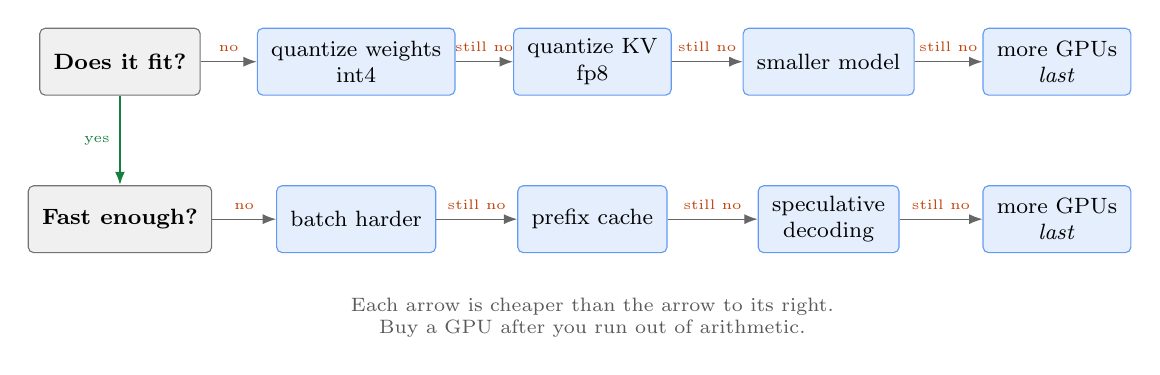
\begin{tikzpicture}[
  font=\scriptsize,
  box/.style={draw=black!55, rounded corners=2pt, fill=black!3,
              minimum height=0.85cm, inner xsep=5pt, align=center,
              font=\footnotesize},
  act/.style={box, fill=accent!12, draw=accent!70},
  q/.style={box, fill=black!6, font=\footnotesize\bfseries},
  ar/.style={-{Latex[length=1.7mm]}, black!60}
]
% --- row 1: does it fit? ---
\node[q]   (fit)  at (0,3.0)   {Does it fit?};
\node[act] (q4)   at (3.0,3.0) {quantize weights\\ int4};
\node[act] (kv)   at (6.0,3.0) {quantize KV\\ fp8};
\node[act] (sm)   at (9.0,3.0) {smaller model};
\node[act] (gpu)  at (11.9,3.0) {more GPUs\\ \emph{last}};

\draw[ar] (fit) -- node[above, font=\tiny, warn] {no} (q4);
\draw[ar] (q4)  -- node[above, font=\tiny, warn] {still no} (kv);
\draw[ar] (kv)  -- node[above, font=\tiny, warn] {still no} (sm);
\draw[ar] (sm)  -- node[above, font=\tiny, warn] {still no} (gpu);

% --- row 2: fast enough? ---
\node[q]   (fast) at (0,1.0)   {Fast enough?};
\node[act] (bat)  at (3.0,1.0) {batch harder};
\node[act] (pre)  at (6.0,1.0) {prefix cache};
\node[act] (spec) at (9.0,1.0) {speculative\\ decoding};
\node[act] (gpu2) at (11.9,1.0) {more GPUs\\ \emph{last}};

\draw[ar] (fast) -- node[above, font=\tiny, warn] {no} (bat);
\draw[ar] (bat)  -- node[above, font=\tiny, warn] {still no} (pre);
\draw[ar] (pre)  -- node[above, font=\tiny, warn] {still no} (spec);
\draw[ar] (spec) -- node[above, font=\tiny, warn] {still no} (gpu2);

\draw[ar, good, thick] (fit.south) -- node[left, font=\tiny, good] {yes} (fast.north);

\node[align=center, font=\scriptsize, black!65] at (6.0,-0.25)
  {Each arrow is cheaper than the arrow to its right.\\
   Buy a GPU after you run out of arithmetic.};
\end{tikzpicture}
\end{center}
\end{frame}
\note{\textbf{32:00.} Photograph-able. Money is the last resort. Most labs buy a card when a flag would have done.}

% -------------------------------------------------------------------------
\begin{frame}{Dollars per million tokens, and when to use an API}
  \begin{equation*}
    \text{\$ per 1M tokens}
      \;=\;
      \frac{\text{GPU \$/hour}}{\text{tokens/sec} \times 3600}
      \times 10^{6}
  \end{equation*}
  \vspace{0.4em}
  \begin{itemize}
    \item \warnc{tokens/sec must be your \emph{aggregate} throughput}, across
          all concurrent requests. So batching is an \emph{economic} decision.
    \item An owned GPU sitting idle costs the same as a busy one.
  \end{itemize}
  \vspace{0.4em}
  \begin{center}
    \begin{minipage}{0.9\textwidth}
      \begin{block}{When self-hosting wins}
        \small
        An API beats self-hosting unless you have
        \textbf{sustained high utilization}, a \textbf{fine-tuned model}, or
        \textbf{data that legally cannot leave the building}.

        \vspace{0.2em}
        Taiwanese manufacturing clients bring the last one often, which is
        why on-prem serving is a job here.
      \end{block}
    \end{minipage}
  \end{center}
\end{frame}
\note{\textbf{33:00.} Notebook Part 5 runs this for any \$/hour you name.
Give them the sentence they can say to a PI: ``at our utilization this costs
X per million tokens; the API costs Y''.}

% -------------------------------------------------------------------------
\begin{frame}{How to benchmark without fooling yourself}
  \begin{enumerate}
    \item \textbf{Warm up first.} The first request pays for CUDA graph
          capture, allocator growth and JIT.
    \item \textbf{Fix the concurrency} and state it. A number without a batch
          size means nothing.
    \item \textbf{Use realistic input \emph{and} output lengths.}
          A 20-token prompt tells you nothing about a RAG deployment.
    \item \textbf{Report TTFT, ITL and throughput together.}
          One of them alone misleads.
    \item \textbf{Re-run the arithmetic} from Parts 1--5 against what the
          server reports. It should line up. If it does not, suspect the
          benchmark first.
  \end{enumerate}
\end{frame}
\note{\textbf{34:00.} Point 5 is the whole talk in one instruction: the
arithmetic is a check on your measurement, and the measurement is a check on
your arithmetic.}

% =========================================================================
% Close (no section page: the checklist speaks for itself)
% =========================================================================

\begin{frame}{Seven steps for your first deployment}
  \vspace{0.2em}
  \begin{enumerate}
    \item \textbf{Compute the weight memory} before you download anything.
    \item \textbf{Compute the KV cache per token}. That is your user capacity.
    \item \textbf{Serve it with vLLM or SGLang.} Skip the for-loop.
    \item \textbf{Quantize to int4}, then re-run \emph{your own} eval.
    \item \textbf{Quantize the KV cache as well.}
    \item \textbf{Cache the prefix} if your prompts share one.
    \item \textbf{Report TTFT, ITL and throughput at a stated concurrency}
          or report nothing.
  \end{enumerate}
  \vspace{0.6em}
  \begin{center}\small
    Steps 1 and 2 need no GPU, no installs and about two minutes.
  \end{center}
\end{frame}
\note{\textbf{35:30.} This is the slide they photograph. Stop talking for three
seconds and let them take it. Then the take-home.}

% -------------------------------------------------------------------------
\begin{frame}{The model you can serve beats the model you cannot}
  \vspace{1.4em}
  \begin{center}
    \begin{minipage}{0.9\textwidth}
      \begin{alertblock}{}
        \centering\large
        The model you can serve is more useful than the model you cannot,
        and memory bandwidth and VRAM decide \emph{which one you can serve}.

        \vspace{0.5em}
        \textbf{You can compute both in advance.}
      \end{alertblock}
    \end{minipage}
  \end{center}
\end{frame}
\note{\textbf{37:00.} Say it once and stop.}

% -------------------------------------------------------------------------
\begin{frame}[fragile]{Questions}
  \vspace{0.6em}
  \begin{center}
    {\Large\bfseries Questions}
  \end{center}
  \vspace{1.2em}
  \begin{center}\small
    Notebook and slides:\\[0.3em]
    \url{https://github.com/Chung-I/MiRA_training_course_2026}\\[0.8em]
    Open the serving demo directly in Colab:\\[0.3em]
    {\scriptsize\url{https://colab.research.google.com/github/Chung-I/MiRA_training_course_2026/blob/main/notebooks/llm_serving_demo.ipynb}}
  \end{center}
  \vspace{0.8em}
  \begin{center}\footnotesize
    Leave this slide up. Parts 1--5 run on a free CPU runtime.
  \end{center}
\end{frame}
\note{\textbf{37:30 to 40:00 for questions.} Leave the checklist slide up
instead of this one if the room is quiet. Backup slides follow.}

% =========================================================================
\appendix
% =========================================================================

\begin{frame}[standout]
  Appendix\\[0.4em]
  {\normalsize Cut candidates, in cut order}
\end{frame}
\note{Not shown unless asked. Cut order comes from the plan: Movement 3d
first, then the tail of the toolbox. Keep Movements 3b and 3c, because
the named engines and the robot contrast are what this room will use.}

% -------------------------------------------------------------------------
\begin{frame}{Backup: none of the three ran from \texttt{pip} on a clean machine}
  \small
  All three install from \texttt{pip}. On an RTX 5090 with no CUDA toolkit,
  \emphc{none of them served from that install}. All three ran in their official
  containers.
  \vspace{0.5em}
  \begin{center}
    \begin{tabular}{lll}
      \toprule
      & \textbf{what broke} & \textbf{why} \\
      \midrule
      vLLM    & \texttt{nvcc} not found        & DeepGEMM wants a toolkit \\
              & \texttt{ninja} not found       & venv \texttt{bin} not on \texttt{PATH} \\
              & compiler/header mismatch       & nvcc 13.3 vs CUDA 13.0 headers \\[0.4em]
      SGLang  & FlashInfer JIT fails           & no \texttt{nvcc}; the wheel ships only \texttt{ptxas} \\[0.4em]
      TRT-LLM & \texttt{libmpi.so.40} missing  & links against system OpenMPI \\
      \bottomrule
    \end{tabular}
  \end{center}
  \vspace{0.6em}
  Both engines wanted a compiler for \textbf{FP8 and JIT paths this fp16
  benchmark never executes}.
  \vspace{0.3em}
  \begin{center}
    \emphc{Run them in their official containers.}
  \end{center}
\end{frame}
\note{Backup only. Use if someone asks "is it really just pip install". The
venv-bin-on-PATH one is the generalizable trap: it fails looking like a missing
dependency when it is a PATH problem.}

% -------------------------------------------------------------------------
\begin{frame}{Backup: five TensorRT-LLM configs, none of them helped}
  \small
  The flat TRT-LLM curve was worth chasing. Resolved config first, guesses
  second:
  \texttt{max\_batch\_size}=2048 (nothing queued), CUDA graphs
  \emph{already on} for \texttt{bs=[1..32,64,128]}, overlap scheduler already on.
  \vspace{0.4em}
  \begin{center}
    \begin{tabular}{lrr}
      \toprule
      \textbf{config} & \textbf{batch 64} & \textbf{vs baseline} \\
      \midrule
      baseline                     & 9,291 & 100\% \\
      FlashInfer attention         & 8,597 & \warnc{93\%} \\
      \texttt{max\_num\_tokens}=32k & 9,318 & 100\% \\
      chunked prefill              & 9,071 & 98\% \\
      KV fraction 0.7              & 9,271 & 100\% \\
      \bottomrule
    \end{tabular}
  \end{center}
  \vspace{0.5em}
  \textbf{Per-request overhead} dominates a 0.5\,B model emitting 128
  tokens, and no flag touches it.
  \vspace{0.3em}
  \begin{center}
    \emphc{A benchmark outside a tool's design envelope measures the envelope.}
  \end{center}
\end{frame}
\note{Backup. The negative result, and the answer to ``why is TRT-LLM last in
your table'': we benchmarked it on the wrong thing and kept it in to make
that point.}

% -------------------------------------------------------------------------
\begin{frame}{\cutbadge{1: cut this first} \; The layer below: Triton, and a training contrast}
  \vspace{0.4em}
  \begin{itemize}
    \item \textbf{Triton} is a Python DSL for GPU kernels. You write
          tile-level code; the compiler handles coalescing, shared memory and
          layout. People now write custom kernels in Triton instead of raw CUDA,
          and it appears \emph{inside} each stack in this talk.
    \item \textbf{Liger-Kernel} is a set of fused Triton kernels (RMSNorm, RoPE,
          SwiGLU, fused linear cross-entropy), claiming $+20\%$ throughput and
          $-60\%$ memory.

          \vspace{0.3em}
          \warnc{For training, not serving.} Mention it only as the contrast:
          the same technique, the other half of the lifecycle.
  \end{itemize}
  \vspace{0.6em}
  \begin{center}\small
    This whole frame is Movement 3d. It is the first thing to drop if the
    talk is running long.
  \end{center}
\end{frame}
\note{One slide, optional, and the first casualty. If you are past 30 minutes
when you reach Movement 3c, you have already skipped this.}

% -------------------------------------------------------------------------
\begin{frame}{\cutbadge{2: trim next} \; \#5 Speculative decoding: 2$\times$, and the same output}
  \begin{itemize}
    \item A \textbf{small draft model} proposes $k$ tokens.
    \item The \textbf{big model verifies all $k$ in a single forward pass}.
    \item Accepted tokens are kept; the first rejection restarts from there.
  \end{itemize}
  \vspace{0.8em}
  \begin{center}
    \begin{minipage}{0.9\textwidth}
      \begin{block}{Why it works, a callback to Movement 2}
        You are \emph{bandwidth-bound}, so you have \emph{spare compute}.
        Verifying $k$ tokens costs roughly one token's worth of weight
        traffic. You are buying speed with compute you were not using.
      \end{block}
    \end{minipage}
  \end{center}
  \vspace{0.6em}
  Typically 1.5--3$\times$ faster, with an \emphc{identical output
  distribution}.
\end{frame}
\note{The identical distribution sets it apart from the other tricks: there
is a proof of zero quality loss. Worth 30 seconds
if you have them.}

% -------------------------------------------------------------------------
\begin{frame}{\cutbadge{2: trim next} \; \#6 A smaller model, and \#7 more GPUs, last}
  \begin{columns}[T]
    \begin{column}{0.49\textwidth}
      \textbf{\#6 Serve a smaller model}\\[0.3em]
      \small
      A distilled or smaller model that \emph{passes your eval} beats a
      big one that is too slow to use.\\[0.5em]
      And: one base model with many \textbf{LoRA adapters} instead of many
      full fine-tunes. The adapters are megabytes; the base model is loaded
      once.\\[0.4em]
      \emph{(Adapters here are a serving trick. Training is another talk.)}
    \end{column}
    \begin{column}{0.49\textwidth}
      \textbf{\#7 More GPUs, last}\\[0.3em]
      \small
      \textbf{Tensor parallel} inside a node; needs a fast interconnect
      (NVLink), or you have moved the bottleneck to the wire.\\[0.5em]
      \textbf{Pipeline parallel} across nodes.\\[0.5em]
      \textbf{CPU offload} as a last resort, and it is slow for the same
      reason decode is slow: PCIe bandwidth is more than an
      order of magnitude below HBM, and decode is bandwidth-bound.
    \end{column}
  \end{columns}
\end{frame}
\note{If you only have one sentence: hardware is the most expensive fix and
the least likely to be necessary.}

% -------------------------------------------------------------------------
\begin{frame}{Backup: the questions that come up}
  \small
  \begin{itemize}
    \item \textbf{Self-host or API?} API, unless sustained high volume, a
          fine-tuned model, or data that cannot leave the building. Do the
          \$/1M math.
    \item \textbf{Does quantization hurt quality?} Sometimes, and not
          uniformly across tasks. 4-bit weight-only holds up on most tasks, but confirm
          on \emph{your} eval, not on perplexity.
    \item \textbf{Why is my model slow on a big GPU?} You are bandwidth-bound
          at batch 1. Batch it, or shrink the bytes.
    \item \textbf{vLLM, SGLang or TensorRT-LLM?} vLLM by default; SGLang for
          structured output and prefix reuse; TensorRT-LLM for the last 20\%
          on fixed NVIDIA hardware.
    \item \textbf{How much VRAM for a 70B?} int4 $\approx$ 35\,GB of weights,
          plus cache. In practice two 40\,GB cards or one 80\,GB card, and
          you will still want a quantized KV cache.
    \item \textbf{CPU offload?} You can, and it will be slow. PCIe is $>10\times$
          below HBM.
    \item \textbf{MoE?} Fewer \emph{active} parameters per token, so faster
          decode, but you still hold \emph{all} the experts in VRAM. Good
          for speed, no help for capacity.
  \end{itemize}
\end{frame}
\note{Do not pre-empt these on the main slides. Let them be asked.}

% -------------------------------------------------------------------------
\begin{frame}{Sources for every number on these slides}
  \small
  \begin{itemize}
    \item \textbf{Llama-3-8B} 32 layers / 8 KV heads / head\_dim 128;
          \textbf{Llama-2-7B} 32 KV heads. From the models' own
          \texttt{config.json}. Notebook Part 2 pulls them live.
    \item \textbf{Capacity table} (7 / 18 / 36 users): notebook Part 3,
          24\,GB card, 8k context, 2\,GB overhead.
    \item \textbf{0.920 vs 0.928\,GB, 169.9 vs 1811.6 tok/s, batch 1
          vs 16}: measured on an RTX 5090 with Qwen2.5-0.5B-Instruct,
          notebook Parts 6--8.
    \item \textbf{20.4--38.2\% KV utilization, 2--4$\times$ throughput,
          1.7--2.7$\times$ Orca, 22$\times$ FasterTransformer}: Kwon et al.,
          arXiv:2309.06180.
    \item \textbf{17.6 / 44.0 / 21.2 / 13.1\,ms}: FlashRT's own reported
          figures. Not reproduced by us.
  \end{itemize}
  \vspace{0.5em}
  \begin{center}\footnotesize
    Bandwidth figures are spec-sheet values (notebook Part 4).
    Prefer a number measured on the card your lab owns.
  \end{center}
\end{frame}
\note{Have this open during questions. Someone will check the KV
arithmetic, and they should.}

\end{document}
